\documentclass[11pt, oneside]{article}   	% use "amsart" instead of "article" for AMSLaTeX format
\usepackage[margin=1in]{geometry}                		% See geometry.pdf to learn the layout options. There are lots.
\geometry{letterpaper}                   		% ... or a4paper or a5paper or ... 
%\geometry{landscape}                		% Activate for rotated page geometry
%\usepackage[parfill]{parskip}    		% Activate to begin paragraphs with an empty line rather than an indent
\usepackage{graphicx}				% Use pdf, png, jpg, or eps§ with pdflatex; use eps in DVI mode
								% TeX will automatically convert eps --> pdf in pdflatex		
\usepackage{amssymb}
%usepackage{undertilde}
\usepackage[numbered,framed]{matlab-prettifier}

\usepackage[T1]{fontenc}
\usepackage{mathtools}  % loads »amsmath«
\usepackage{physics}
\usepackage{listings}


\setlength{\parskip}{0.5em}

%SetFonts
\newcommand\Rey{\mbox{\textit{Re}}}

\title{\vspace{-6ex} Assignment 1- Molecular Dynamics \\ {CSCI 596: Scientific Computing \& Visualization}  \vspace{-2ex}}
\author{Anup V Kanale}
\date{\vspace{-3ex}\today}							% Activate to display a given date or no date

\begin{document}
\maketitle

\section{Scaling using Linked-List MD}
In this section, we shall compare the effect of scaling on the linked-list cell implementation program \texttt{lmd.c}, and the regular molecular dynamics program \texttt{md.c}. The two programs were run for different number of unit cells \texttt{InitUcell} (from \{4,4,4\} to \{10,10,10\}). The corresponding number of atoms,  \texttt{nAtom} is calculated as $ \text{nAtoms} = 4 \text{atoms/cell} * (\text{InitUcell})^3 \text{cells}$, and it varies from 256 to 4000.

The time of execution $T$ was measured for each case and fit as per the formula $T = C \times (\text{nAtoms})^p$. Upon taking the logarithm, we see that $\log T = p \log (\text{nAtoms}) + K$. Therefore, the slope of the line in the log plot gives us the order of scaling.  The results are summarized in the plot below.

As we can see from the equations of fit lines, the regular md program scales almost quadratically, whereas the linked-list cell implementation scales linearly with the number of atoms. This agrees with the theoretical prediction.
\begin{figure} [!htbp]
	\centering
	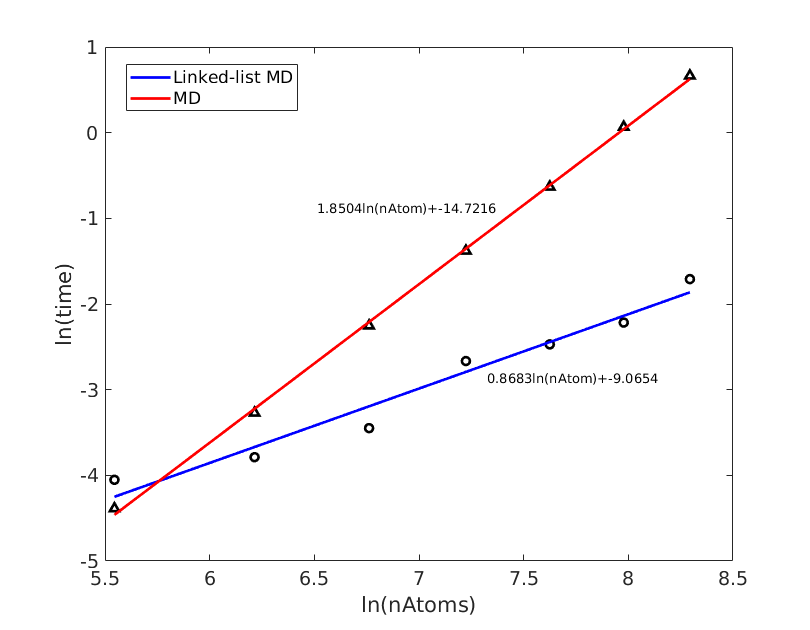
\includegraphics[scale=0.5]{mdVsLmd.png}
	\caption{Scaling of regular and linked-list MD programs}
\end{figure}

\section{Flop/s Performance}
Performance of a program is often measured in MFlop/s (megaflop/s = million floating point operations per second). To get a "\textit{feel}" of this performance measure, the linked-list md program \texttt{lmd.c} was run for \texttt{InitUcell} = \{10,10,10\} (or \texttt{nAtom} = 4000). The number of floating point operations ($+$, $-$, $*$, $/$) executed were counted and this result was divided by the value obtained for elapsed time (in seconds) to obtain the program's Mflop/s performance. (for simplicity, sqrt() counts as 1 operation).

This test was performed on a laptop with Intel core i5 processor with a clock speed of 2.3GHz. The results obtained were as follows:
\begin{itemize}
	\item \textbf{Execution time}: $1.787950E-01$ s
	\item \textbf{Number of floating-point operations}: $1.506044E+08$
	\item \textbf{Mflop/s performance}: $8.423302E+02$
\end{itemize}

\appendix
\section{Programs}
A python script was written to automate the running of the programs for different values of \texttt{InitUcell}. The script is as shown below.
\lstinputlisting[language=Python, frame=single]{autoAssgn1.py}

The matlab script used to generate these plots is shown below.
	\lstinputlisting[style=Matlab-editor]{plotgen.m}
\end{document}